
\documentclass[letterpaper, 11pt]{article}
\usepackage[utf8]{inputenc}
\usepackage{titlesec}
\usepackage{fullpage} % changes the margin
\usepackage{graphicx} %package to manage images
\graphicspath{ {./images/} }
\usepackage{algpseudocode}
\usepackage{algorithm}

\begin{document}
\begin{titlepage}
\vspace*{0.7in}
\begin{center}
\begin{figure}[htb]
\begin{center}

\includegraphics[width=8cm]{univ_logo}
\end{center}
\end{figure}
\vspace*{0.3in}
\begin{Large}
\textbf{SOEN 6011 : SOFTWARE ENGINEERING PROCESSES} \\
\end{Large}
\vspace*{0.1in}
\begin{Large}
\textbf{SUMMER 2022} \\
\end{Large}
\vspace*{0.9in}
\begin{Large}
\textbf{ETERNITY} \\
\end{Large}
\vspace*{0.625in}
\begin{Large} 

\textbf{PROBLEM - 1} \\
\vspace*{0.2in}
Function Description\\
\vspace*{0.1in}
\end{Large}
\vspace*{0.625in}
\rule{80mm}{0.1mm}\\
\vspace*{0.1in}
\begin{large}
Author \\
\vspace*{0.1in}
Neona Sheetal Pinto\\
\vspace*{1.0in}
\date{\normalsize\today} 
\end{large}
\end{center}
\begin{center}
https://www.overleaf.com/project/62e9f079b389ca1bdb5b238c\end{center}

\end{titlepage}


\tableofcontents
\listofalgorithms


\newpage

\section{
    {PROBLEM 3 - F6: $B(x, y)$}}

    \subsection{Algorithm Description and Pseudo-Code}
        \normalsize {SOEN 6011 - Summer 2022}
        \\
    \subsection{Mind-map for pseudo-code format decision} 
        The figure \ref{fig:mindmap}  shows the mind-map showcasing features supported by various algorithm/pseudo-code packages in Latex. The  mind-map shows how most of the features are supported by almost all the packages. The {$Customization$} feature highlighted in red block is a powerful feature which provides flexibility in adding new customised features which is supported by \textbf{algpseudocode $+$ algorithmicx}, Hence the  reason in choosing the {$Customization$} format for representing the algorithms in this document.\cite{Pseudo-code}
        \\\\\\\
    \begin{figure}[htb]
        \begin{center}
            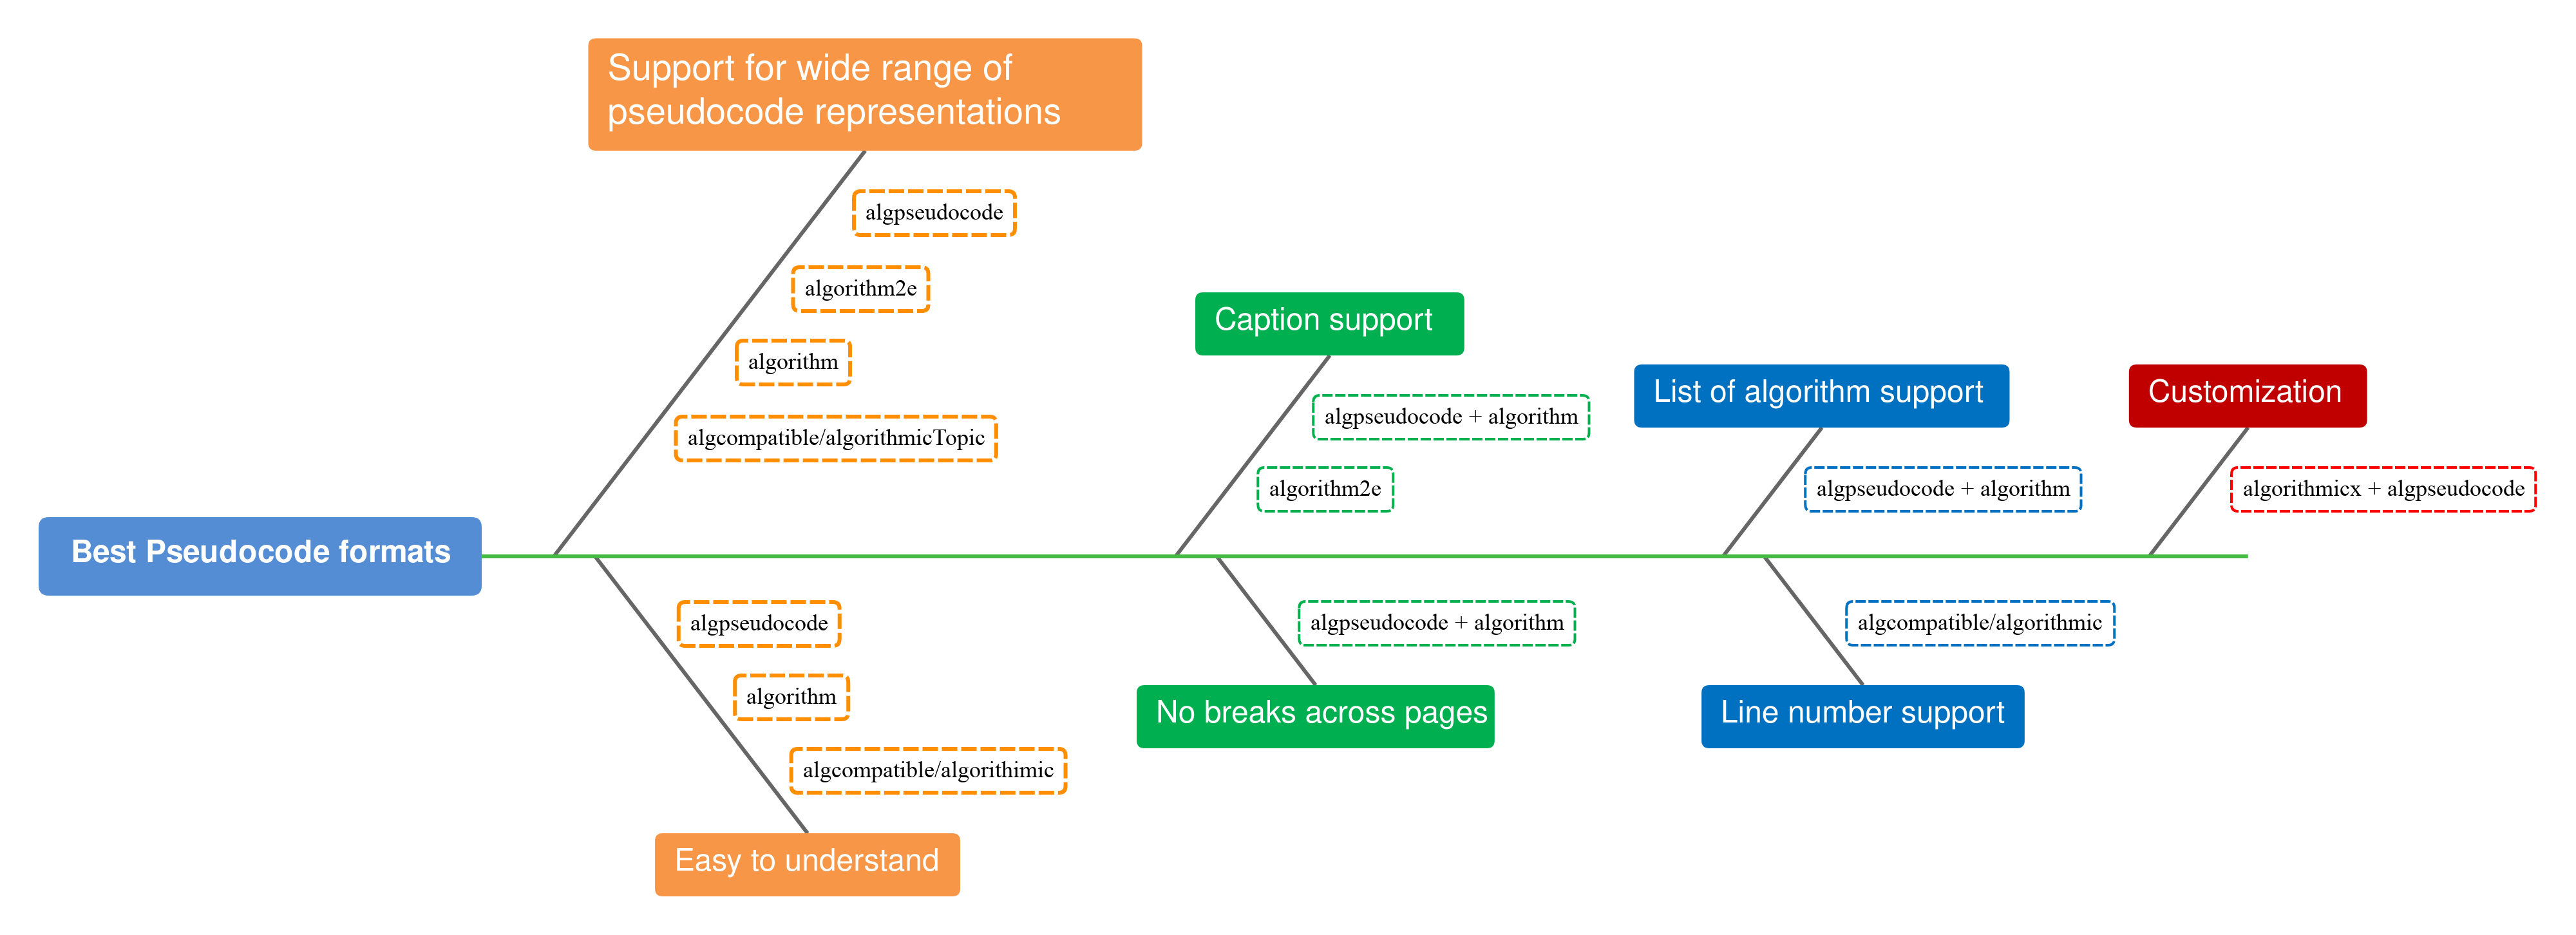
\includegraphics[width=18cm]{images/mindmap_pseudo.png}
        \end{center}
        \caption{Mind map for pseudocode format decision}
        \label{fig:mindmap}
    \end{figure}
    \newpage
    \subsection{Algorithms for Beta function:}
    The following are the ways to find Beta value of the given variables (x,y):
        \begin{itemize}
            \item \textbf{Algorithm 1: Trapezoidal Rule} 
                The trapezoidal rule chooses points in [a,b] starting with a and ending with b. Trapezoidal Rule is a rule that evaluates the area under the curves by dividing the total area into smaller trapezoids rather than using rectangles. This integration works by approximating the region under the graph of a function as a trapezoid, and it calculates the area. This rule takes the average of the left and the right sum \cite{trapezoidal2}
                \item Let f(x) be a continuous function on the interval [a, b]. Now divide the intervals [a, b] into n equal sub intervals with each of width,
                
                ${\Delta}$ $x = (b-a)/n, t a = x0 < x1< x2< x3<…..<xn = b$
                
                Then the Trapezoidal Rule formula for area approximating the definite integral
                \(\int_{a}^{b}f(x)\,dx\)
                
                \(\int_{a}^{b}f(x)dx\approx T\_{n}=\frac{\bigtriangleup x}{2}[f(x_{0})+ 2f(x_{1})+2f(x_{2})+….2f(x_{n-1})+f(x_{n})]\)
                
                Where, $xi = a+i{\Delta}x$
                
                If n →$\infty$, R.H.S of the expression approaches the definite integral
                \begin{center}
                    \(\int_{a}^{b}f(x)\,dx\)    
                \end{center}
                
                \item
                The name trapezoidal is because when the area under the curve is evaluated, then the total area is divided into small trapezoids instead of rectangles. Then we find the area of these small trapezoids in a definite interval.
                
                \item \textbf{Algorithm 2: Simpson's Rule}  
                In numerical analysis, Simpson’s rule is a method for numerical approximation of definite integrals. Specifically, it is the following approximation: 

                $$\int_{a}^{b} f(x) dx \approx \frac{(b-a)}{6} \bigg(f(a) + 4f \frac{(a+b)}{2} + f(b)\bigg)$$    
                
                In Simpson’s 1/3 Rule, we use parabolas to approximate each part of the curve.We divide 
                the area into n equal segments of width $\mathbf{\Delta x}.$
                Simpson’s rule can be derived by approximating the integrand f (x) (in blue) 
                by the quadratic interpolant P(x).
                \item In order to integrate any function f(x) in the interval (a, b), follow the steps given below:
                1.Select a value for n, which is the number of parts the interval is divided into. 
                2.Calculate the width, h = (b-a)/n 
                3.Calculate the values of x0 to xn as x0 = a, x1 = x0 + h, …..xn-1 = xn-2 + h, xn = b. 
                Consider y = f(x). Now find the values of y(y0 to yn) for the corresponding x(x0 to xn) values. 
                4.Substitute all the above found values in the Simpson’s Rule Formula to calculate the integral value.
                Approximate value of the integral can be given by Simpson’s Rule: 
                
                  $$\int_{a}^{b} f(x) dx \approx \frac{h}{3} \bigg(f_0 + f_n + 4 * \sum_{i=1,3,5}^{n-1}f_i + 2* \sum_{i=2,4,6}^{n-2}f_i \bigg)$$ \cite{simpson1}   
        \end{itemize}
        \subsection{\textbf{Technical Reasons for selecting Trapezoidal Integration for calculating the definite integral of the Beta function: }}
        \textbf{Advantages: }
        \begin{itemize}
            \item It requires less steps than the rectangular method to get the same accuracy so it is somewhat faster on a computer.
            \item The trapezoidal method is a little more complicated but is still relatively easy to understand.
            \item
            The trapezoidal rule is mostly used in the numerical analysis process as they provide more     accurate results.
            \item Trapezoid rule is its rather easy conceptualization and derivation. \cite{trapezoidal3}

        \end{itemize}
        \textbf{Disadvantages: }
        \begin{itemize}
            \item The Trapezoidal Rule does not give accurate value as Simpson’s Rule when the underlying function is smooth 
            \item It follows that if the integrand is concave up (and thus has a positive second derivative), then the error is negative and the trapezoidal rule overestimates the true value.
        \end{itemize} 
    \textbf{Therefore, the reasons above show the use of trapezoidal rule for calculating the definite integral in the Beta function.}\\
    
    \newpage
    
    \subsection{Pseudo Code for Trapezoidal rule for the definite integral to calculate Beta function}
            \subsubsection{Description}
            To find the area from a to b , we can divide the area into n trapezoids, and the width of each trapezoid is w, so we can say that (b - a) = nw. When the number of trapezoids increases, the result of area calculation will be more accurate. The function passed inside the integral is what produces the Beta function output.\cite{trapezoidal1}
            \subsubsection{Algorithm : Trapezoidal rule of Integral to calculate Beta function - algorithm\ref{exp3}}
                \begin{algorithm}
                    \caption{Trapezoidal rule for definite integral}\label{exp3}
                    \begin{algorithmic}[1]
                        \Require $x > 0$ AND $y > 0, x, y \in R$
                        
                        \Function{Integral}{$a, b, x, y$}\Comment{algorithm for ${\displaystyle \mathrm \int_{0}^{1}t^{x-1}(1-t)^{y-1}\,dt}$}
                        \State $area\gets 0$
                        \State $modifier\gets 1$
                        \State $a\gets 0$
                        \State $b\gets 1$
                            \For{$i \gets a + increment, i < b , i \gets i + increment $} \Comment{increment is equal to 1E-4}
                                \State $dist \gets i - a$
                                \State $f1 \gets \Call{Exponential}{a + dist - increment, x,y}$
                                \State $f2 \gets \Call {Exponential}{a + dist - increment, x,y}$
                                \State $area = area + increment/2  * f1 + f2$ 
                            \EndFor \\
                        \Return $area * modifier$
                        \EndFunction
                    \end{algorithmic}
                \end{algorithm}
    \newpage       
    \subsection{Pseudo Code for Simpson's rule for the definite integral}
            \subsubsection{Description}
                Simpson's Rule is based on the fact that given three points, we can find the equation of a quadratic through those points. The function passed inside the integral is what produces the Beta function output.
            \subsubsection{Algorithm : Simpson's - algorithm\ref{exp2}}
                \begin{algorithm}
                    \caption{Simpson's rule for definite integral}\label{exp2}
                    \begin{algorithmic}[1]
                        \Require $x > 0$ AND $y > 0, x, y \in R$
                        
                        \Function{Integral}{$a, b, x, y$}\Comment{algorithm for ${\displaystyle \mathrm \int_{0}^{1}t^{x-1}(1-t)^{y-1}\,dt}$}
                              \State $number \gets 10000$  \Comment{precision parameter}
                              \State $w \gets (b - a) / (number - 1)$ \Comment{Step size}
                              \State $sum \gets 1.0 / 3.0 * \Call{Exponential}{x,y} + \Call{Exponential}{x,y}$
                              \For{$i \gets 1; i < number - 1; i \gets i + 2)$ }
                                 \State $x \gets a + w * i$
                                 \State $sum \gets sum + 4.0 / 3.0 * \Call{Exponential}{x,y}$
                              \EndFor
                              \For{$i \gets 2; i < number - 1; i \gets i + 2)$ }
                                 \State $x \gets a + w * i$
                                 \State $sum \gets sum + 2.0 / 3.0 * \Call{Exponential}{x,y}$
                              \EndFor
                              \Return $sum * w$;
                
                        \EndFunction
                    \end{algorithmic}
                \end{algorithm}
                
    \subsection{Pseudo Code for Taylor's Series for calculating Exponential value}
            \subsubsection{Description}
            Taylor series is a representation of a function as an infinite sum of terms that are calculated from the values of the function's derivatives at a single point.
            This is a sub function used in Beta function for calculating the definite integral. There are 2 utility functions used by the main function exponent to calculate the $x^y$ 
            \subsubsection{Algorithm : Exponent - algorithm\ref{exp1}}
                \begin{algorithm}
                    \label{alg:3}
                    \caption{Exponentiation by Taylor Series}\label{exp1}
                    \begin{algorithmic}[1]
                        \Require $x \neq 0$ AND $y > 0$
                        
                        \Function{Exponent}{$base, power$}\Comment{algorithm for $x^y$ considering all conditions and using sub functions}
                            \State $result \gets 1$
                            \State $roots \gets 1$
                            \State $base\_value \gets x$
                            \State $power \gets y$ \Comment{Power is integer simply multiply and return result}
                            \If{$power\_value \% 1  \equiv 0$}
                                \For{$counter <= power\_value$}
                                    \State {$result \gets result * x$}
                                \EndFor \Comment {Power is a decimal number}
                            \Else 
                                \If{$power\_value >= 1$}
                                    \State $exponent\_value[] \gets \Call{Exponential}{base\_value, power\_value}$
                                    \State $roots = roots * exponential\_value[0]$
                                    \State $power\_value \gets exponential\_value[1]$
                                \EndIf
                            \EndIf 
                             \If{$power\_value > 0$ AND $power\_value < 1$}
                                \State{$precision \gets 1$}
                                \State {$findroot \gets \Call{findClosestRoot}{base\_value, den,0, precision}$}
                                \While{$base\_value < \Call{Exponential}{findroot, den}$ AND $precision > 0.000001$}
                                    \State{$findroot \gets findroot - precision$}
                                    \State{$precision \gets precision * 0.1$}
                                    \State{$findroot \gets \Call{findClosestRoot}{base\_value, den, findroot, precision}$}
                                \EndWhile
                                \State {$value \gets \Call{Exponential}{findroot, power\_value * den}[0]$}
                                \State{$roots \gets roots * value$}
                                \State{$result \gets root$}
                            \EndIf  \\
                            \Return result
                        \EndFunction
                        
                        \Function{findClosestRoot}{$base, power, root, precision$}\Comment{algorithm for finding the root with closest precision}
                            \State $closestRoot \gets closestRoot +  precision;$
                            \State $temp \gets \Call{Exponential}{closestRoot, power}$
                            \While{$temp[0] < base$}
                                \State $closestRoot \gets closestRoot +  precision;$
                                  \State $temp \gets \Call{Exponential}{closestRoot, power}$
                            \EndWhile \\ 
                            \Return $closestRoot$
                        \EndFunction
                        
                        \Function{exponential}{$x, y$}\Comment{algorithm for $x ^ y$}
                            \State $exponent\_value\gets 1$
                            \While{$power > 0$}
                                \State $exponent\_value\gets exponent\_value * base$
                                \State $power \gets power - 1$
                                \If{$power < 1$}
                                    \State $break$;
                                \EndIf
                            \EndWhile \\ 
                            \Return $exponent, power$
                        \EndFunction
                        
                    \end{algorithmic}
                \end{algorithm}    
           
    \subsection{Annexure:}
        \begin{itemize}
          \item \textbf{Trello Board :} \textit{https://trello.com/eternity119}
          \item \textbf{Code Version Control :} \textit{https://github.com/neonapinto/Scientific\_calculator}
          \item \textbf{Overleaf :} \textit{https://www.overleaf.com/project/62e9f079b389ca1bdb5b238c}
    \end{itemize}
  
\begin{thebibliography}{}      
\bibitem{UniversityLogo} 
Concordia Logo : The logo of Concordia University with transparent background
\\\texttt{https://www.pngwing.com/en/free-png-djpzn}

\bibitem{LatexGuide}
Latex Guidelines : How to write robust and effective latex documents
\\\texttt{https://medium.com/@pbeliveau/latex-coding-standards-f82743b7866b}

\bibitem{trapezoidal1} 
Trapezoidal Rule for definite integral
\\\texttt{https://www.tutorialspoint.com/Trapezoidal-Rule-for-definite-integral}

\bibitem{simpson1} 
Simpson Rule for definite integral
\\\texttt{https://www.javatpoint.com/simpson-method}

\bibitem{trapezoidal2} 
Trapezoidal Rule for definite integral
\\\texttt{https://byjus.com/maths/trapezoidal-rule/}

\bibitem{trapezoidal3} 
8 Difference Between Trapezoidal Rule And Simpson’s Rule In Surveying 
\\\texttt{https://vivadifferences.com/difference-between-trapezoidal-rule-and-simpsons-rule-in-surveying/}


\bibitem{Pseudo-code} 
Pseudo-code in Latex: Different packages to represent algorithm or pseudo-code in latex.
\\\texttt{https://www.overleaf.com/learn/latex/Algorithms}

\end{thebibliography}  

\end{document}